\documentclass[11pt]{article}
\usepackage[letterpaper,margin=1in]{geometry}
\usepackage[T1]{fontenc}
\usepackage{lmodern}
\usepackage{microtype}
\usepackage{amsmath,amssymb}
\usepackage{booktabs}
\usepackage{graphicx}
\usepackage{xcolor}
\usepackage[numbers,sort&compress]{natbib}
\usepackage[hidelinks]{hyperref}
\usepackage{url}
% generated by gen_tables.py -- do not edit
\newcommand{\boardtable}{%
\begin{tabular}{llrrrrl}\toprule
Board & Tier & Cu & Parts & Pair nets & To route & Interfaces\\\midrule
SI test board & easy & 4 & 28 & 2 & 107 & 50\,$\Omega$ lines\\
M.2 PCIe adapter & easy & 4 & 20 & 18 & 93 & PCIe x4\\
HDMI--MIPI bridge & easy & 4 & 121 & 36 & 304 & HDMI, CSI-2\\
GMSL deserializer & medium & 4 & 236 & 28 & 413 & GMSL2, CSI-2\\
Jetson Orin baseboard & medium & 8 & 680 & 208 & 1,625 & PCIe, USB3, CSI-2\\
RDIMM DDR4 tester & hard & 12 & 691 & 226 & 2,021 & DDR4\\
SO-DIMM DDR5 tester & hard & 12 & 706 & 102 & 1,770 & DDR5\\
RDIMM DDR5 tester & hard & 12 & 797 & 178 & 2,300 & DDR5\\
\bottomrule\end{tabular}}

\newcommand{\baselinetable}{%
\begin{tabular}{lrrrrrrrr}\toprule
Board & Time (s) & Compl. & DRC & Skew & Length & Width & Eff. & Reward\\\midrule
SI test board & 54 & 0.90 & 1.00 & 0.00 & 1.00 & 0.00 & 1.00 & \textbf{0.48}\\
M.2 PCIe adapter & 112 & 0.96 & 0.18 & 0.11 & 0.00 & 0.43 & 1.00 & \textbf{0.27}\\
HDMI--MIPI bridge & 181 & 0.18 & 0.34 & 0.00 & 0.00 & 0.00 & 1.00 & \textbf{0.01}\\
GMSL deserializer & 534 & 0.72 & 0.08 & 0.29 & 0.00 & 0.00 & 1.00 & \textbf{0.13}\\
\bottomrule\end{tabular}}

\newcommand{\forecasttable}{%
\begin{tabular}{rccc}\toprule
Budget & 4 h & 1 day & 1 week\\\midrule
\$100 & 0.71 / 0.61 & 0.78 / 0.66 & 0.78 / 0.66\\
\$1,000 & 0.71 / 0.61 & 0.82 / 0.70 & 0.84 / 0.79\\
\$10,000 & 0.71 / 0.61 & 0.82 / 0.70 & 0.84 / 0.82\\
\bottomrule\end{tabular}}

\newcommand{\noracle}{8}\newcommand{\noracleall}{8}\newcommand{\nruns}{18}\newcommand{\nbaseboards}{4}


\title{Routed Is Not Right: A Gold-Master Benchmark for\\ Machine Routing of High-Frequency Printed Circuit Boards}
\author{Dave Rauchwerk\\ Rauchwerk Research\\ \texttt{dbrauchwerk@gmail.com}}
\date{November 2026}

\begin{document}
\maketitle

\begin{abstract}
Learning-based placement and routing for printed circuit boards (PCBs) is usually evaluated on wirelength, via count and design-rule violations. None of the public PCB benchmarks we found scores the properties that make a high-frequency board work: impedance-controlled widths, intra-pair skew and length matching. We introduce \textsc{PCB Gold-Master Eval}, a benchmark of eight fabricated, Apache-licensed boards by Antmicro (4--12 copper layers, 20--797 components, PCIe, MIPI CSI-2, HDMI, GMSL2, DDR4 and DDR5 interfaces). Each task strips the routed copper from a board pinned by commit and checksum, asks an agent or algorithm to route it without moving parts, and scores the result against the human original. Because the designers' length and skew targets are not written in any rule file, the verifier derives them from the human copper itself. Tasks are packaged in the Harbor format; an oracle that restores the human copper scores 1.00 on \noracle{} of \noracleall{} tasks. A Freerouting~2.5 baseline completes 72--96\% of connections on boards without dense BGAs and stalls on a BGA board, and scores far below the human boards on skew, length and width conformance. We pair the benchmark with a graded review of thirty sources, a scored inventory of open-source tools, and a parametric forecast of benchmark reward against compute budget and wall-clock time, which suggests that for open-source stacks the evaluator, not compute, limits progress. Code, tasks and forecast are released under Apache-2.0.
\end{abstract}

\section{Introduction}
Automated routers have long completed PCBs; the hard part of a modern board is completing it \emph{correctly} at high frequency. A DDR5 byte lane, a PCIe link or a MIPI CSI-2 lane works only if its traces keep a controlled impedance on every layer, the two halves of each differential pair arrive within a few picoseconds of each other, and groups of signals are matched in length. Experienced designers meet these constraints by hand, often with serpentine meanders tuned to fractions of a millimetre.

Recent work proposes that machine learning---reinforcement learning (RL), evolutionary search, graph networks and large language models (LLMs)---can learn to place and route boards for such constraints without hand-written heuristics. The evidence is thin. The best-known RL placement result \citep{mirhoseini2021graph} remains disputed after an independent reassessment \citep{cheng2023assessment,goldie2024chip,markov2024reevaluating}. Published PCB routing benchmarks score wirelength, vias and design-rule checks (DRC) \citep{song2026pcbworld}, and none of the learned PCB methods we found optimises signal integrity (SI) end to end. A method cannot be shown to work on a property that is not measured.

This paper contributes:
\begin{enumerate}
\item \textbf{A gold-master benchmark.} Eight fabricated open-hardware boards, stripped of copper, with the human layout as the answer key and a reward that includes pair skew, length-group spread and impedance-width conformance (Section~\ref{sec:bench}).
\item \textbf{Reproducible packaging.} Harbor tasks \citep{harbor} with every input pinned (image digest, board commit, file checksums), a separate verifier sandbox, an oracle, and an integrity signal for runs that copy the public gold layout (Section~\ref{sec:impl}).
\item \textbf{Baselines and a compute forecast.} A Freerouting baseline on the full set, and a parametric model of reward against dollars and hours built from published scaling evidence and measured costs (Sections~\ref{sec:results}--\ref{sec:forecast}).
\end{enumerate}

\section{Related work}
\paragraph{Chip placement with learning.} Graph-based RL for macro placement \citep{mirhoseini2021graph} reported human-competitive floorplans; an independent study found simulated annealing equal or better at roughly one twentieth of the CPU-hours, with weak rank correlation between the proxy cost and routed wirelength or timing \citep{cheng2023assessment}. Black-box and tree-search methods \citep{shi2023wiremask,geng2024efficientplace} and offline RL \citep{lai2023chipformer} outperform earlier RL placers \citep{lai2022maskplace} at hour scale, and GPU analytical placement \citep{lin2019dreamplace} remains fast and strong. ChiPBench \citep{wang2024chipbench} showed that leading on intermediate metrics need not improve final power, performance and area---the central motivation for scoring against end results.

\paragraph{PCB placement and routing.} RL placement of PCB components with adaptive rewards reduced post-route wirelength by 17--21\% against simulated annealing \citep{vassallo2024learning}. Ranking Cost learns cost maps for an A$^*$ router with evolution strategies \citep{huang2021rankingcost}. PCBWorld provides a KiCad-based RL routing environment over 679 real boards, where policies trained on synthetic boards approach rule-based routers on easy splits but trail them on harder ones \citep{song2026pcbworld}. Koppar's autorouter-bench compares routers on public KiCad boards, including several by Antmicro, by open connections, DRC errors and time \citep{zap25}. None of these scores impedance, skew or length matching.

\paragraph{LLM-driven program evolution.} FunSearch \citep{romeraparedes2024funsearch} and AlphaEvolve \citep{novikov2025alphaevolve} evolve programs scored by automated evaluators. In placement, LLM-evolved optimisers improved half-perimeter wirelength by 5--8\% \citep{yao2025evolution}, and HELIX evolved placement heuristics inside OpenROAD for 4.5\% (global) and 5.6\% (routed) geometric-mean wirelength gains at roughly \$250--300 per run \citep{kahng2026helix}.

\paragraph{SI surrogates.} Deep networks predict PDN impedance $>$100$\times$ faster than boundary-element simulation \citep{zhang2021pdn}, and buffer-parameterised surrogates predict eye metrics across technologies with large speedups over simulation \citep{withoft2026surrogate}. Their generalisation beyond trained topologies is not yet established. Antmicro's gerber2ems turns fabrication files into openEMS full-wave models \citep{gerber2ems}.

\section{Benchmark}\label{sec:bench}
\subsection{Gold-master boards}
We selected eight KiCad boards from Antmicro's open-hardware portfolio (Table~\ref{tab:boards}). Selection favoured (i) real high-speed interfaces, (ii) evidence that the board was fabricated and used---measured VNA data, photographs, commercial sale or published research use---and (iii) a spread of size. All are Apache-2.0. Boards are fetched at pinned commits and verified by SHA-256; nothing is redistributed.

\begin{table}[t]
\centering\small
\boardtable
\caption{The gold-master set. \emph{To route}: unconnected connections after stripping, from KiCad's connectivity engine. Tiers reflect layer count, size and interface difficulty.}
\label{tab:boards}
\end{table}

A notable property of the set is that none of Antmicro's rule files (\texttt{.kicad\_dru}) contains length or skew limits; they define per-layer widths and gaps for impedance classes only. The matching the designers achieved lives only in their copper---for example, the DDR4 tester carries 5,514 hand-drawn meander arcs. Scoring against the copper therefore captures intent that no rule file states.

\subsection{Task}
Each task provides a board with all tracks, arcs, vias, tuning patterns and zone fills removed, with placement, footprints, nets, net classes, zone outlines and rules unchanged. The agent must save a routed board in place without moving, rotating, flipping, adding or deleting footprints. The environment supplies KiCad~10.0.7 (with \texttt{pcbnew} Python bindings), Java~25, Freerouting~2.5.0 \citep{freerouting} and network access for other tools.

\subsection{Reward}
Let $u_0$, $u_g$ and $u_c$ be the unconnected counts of the stripped, gold and candidate boards after a zone refill. The reward is
\begin{equation}
R = P \cdot C^2 \cdot \left(0.30\,D + 0.25\,S + 0.15\,L + 0.15\,W + 0.15\,E\right),
\end{equation}
where $P\in\{0,1\}$ gates on untouched placement; $C = 1-(u_c-u_g)/(u_0-u_g)$ is completion; $D = 1/(1+x/10)$ penalises $x$ DRC errors in excess of the gold board's own, by type; $S$ is the fraction of differential pairs whose skew is within $\max(0.15\,\text{mm},\,1.5\times$ the gold skew$)$; $L$ is the fraction of non-default net classes whose length spread is within $\max(1.25\times,\,+1\,\text{mm})$ of the gold spread; $W$ is the fraction of controlled-impedance copper whose width matches a width the designers used for that class on that layer (within 5\,$\mu$m); and $E$ averages the gold-to-candidate ratios of total copper length and via count, capped at 1. Squaring $C$ keeps unfinished boards from scoring well on the quality terms. The verifier also reports $F$, the fraction of candidate segments coincident with gold segments on a 10\,$\mu$m grid; independent routing essentially never reproduces human geometry, so runs with $F>0.5$ are disqualified from leaderboards.

\section{Implementation}\label{sec:impl}
Tasks follow the Harbor format \citep{harbor}: \texttt{instruction.md}, \texttt{task.toml}, an environment Dockerfile, an oracle \texttt{solve.sh} and a verifier \texttt{test.sh}. The Dockerfile fetches the gold board, strips it and deletes it in a single image layer, so the gold copper exists in no layer the agent can read. The verifier runs in a separate sandbox, re-fetches the gold board at the pinned commit, checks its checksum, refills zones and scores. Two engineering findings are worth recording. First, \texttt{kicad-cli}'s DRC report stops listing unconnected items at 499, so completion must be counted with KiCad's connectivity engine instead; a stripped DDR5 board has 2,300. Second, removing items through the \texttt{pcbnew} SWIG bindings crashed in KiCad~10.0.7, so stripping is done on the normalised text representation. All tools, pins and the forecast are driven by a single \texttt{Makefile}.

\section{Results}\label{sec:results}
\paragraph{Oracle.} Restoring the human copper scores $R=1.00$ on \noracle{} of \noracleall{} tasks through Harbor~0.25.0, confirming that the verifier accepts the answer key on every board, including the 12-layer DDR boards.

\paragraph{Freerouting baseline.} Table~\ref{tab:base} reports the best of \nruns{} Freerouting runs (pass limits 1, 3 and 10; two seeds) on each board with results so far. Runs used one CPU core under x86 emulation on an Apple-silicon laptop. On the HDMI--MIPI bridge, Freerouting stalled at 181 unrouted items in its own count after one and after three passes, leaving most of the board's BGA fan-out unrouted; published DDR3 BGA routing cases report the same limitation. Results also vary between runs: on the M.2 adapter, reward ranged from 0.21 to 0.27 across seeds and pass limits. Independent runs overlapped the gold copper by about 1\% ($F$ between 0.008 and 0.012), far below the disqualification threshold. On the eight-layer Jetson Orin baseboard (1,625 connections), neither the one-pass nor the three-pass run finished within the 90-minute limit under emulation; it and the hard tier will be run on native hardware. Where it completes the board, the router still fails the high-frequency terms: on the M.2 PCIe adapter it made 92\% of connections, met the skew tolerance on one of nine pairs and used an impedance-correct width on 40\% of high-speed copper.

\begin{table}[t]
\centering\small
\baselinetable
\caption{Freerouting~2.5 against the gold masters (1.00 = the human original). Columns are the reward terms of Section~\ref{sec:bench}.}
\label{tab:base}
\end{table}

\section{A compute forecast}\label{sec:forecast}
To guide investment we model the reward a strategy reaches with budget $B$ and wall clock $T$. Each strategy has a fixed cost $(B_0,T_0)$, a per-candidate cost $c$ and duration $\tau$, and a parallelism limit $p$; the number of candidates is $N=\min\left((B-B_0)/c,\;(T-T_0)\,p/\tau\right)$ and
\begin{equation}
G(N) = g_0 + (g_{\max}-g_0)\left(1-(1+N/n_0)^{-\alpha}\right).
\end{equation}
With $\alpha=0.6$ and $n_0=60$ the curve reproduces WireMask-EA's observation that 73\% of the final gain arrives within the first 300 of 2,000 evaluations \citep{shi2023wiremask}. Starting points come from the measured baselines; per-candidate costs from the baselines and on-demand prices on 7 November 2026; LLM-evolution costs from HELIX \citep{kahng2026helix}; RL fixed costs from the reassessment of \citet{cheng2023assessment}; and ceilings for untested strategies are explicit assumptions, tagged in the released parameter file. Figure~\ref{fig:surface} shows the best achievable reward on the hard tier and Table~\ref{tab:fc} summarises both tiers.

\begin{figure}[t]
\centering
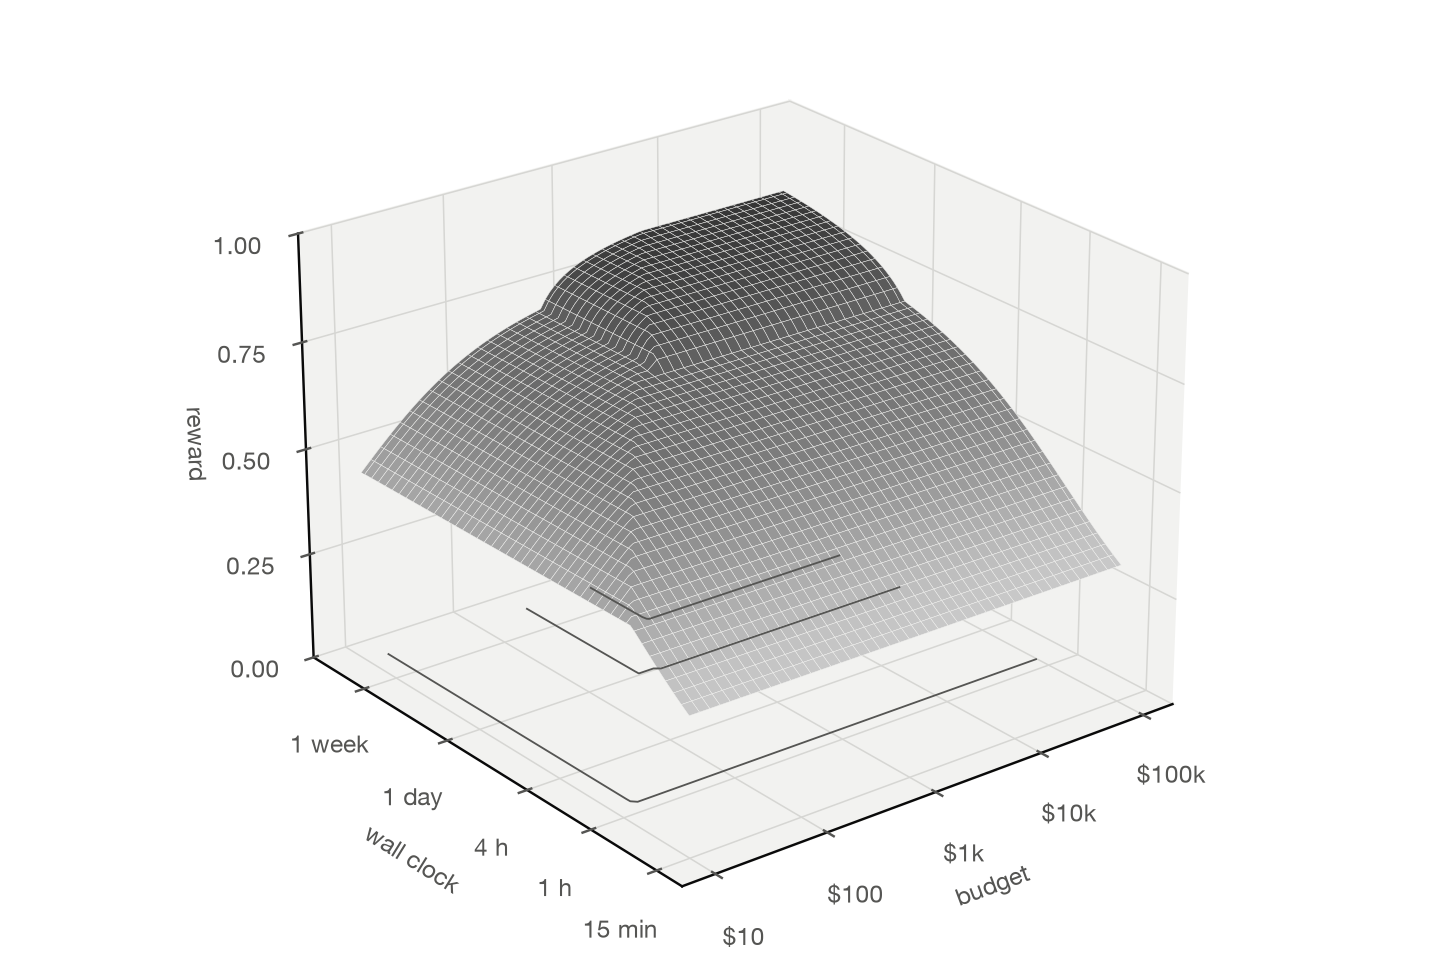
\includegraphics[width=0.62\linewidth]{fig/fc_surface3d_hard.png}\hfill
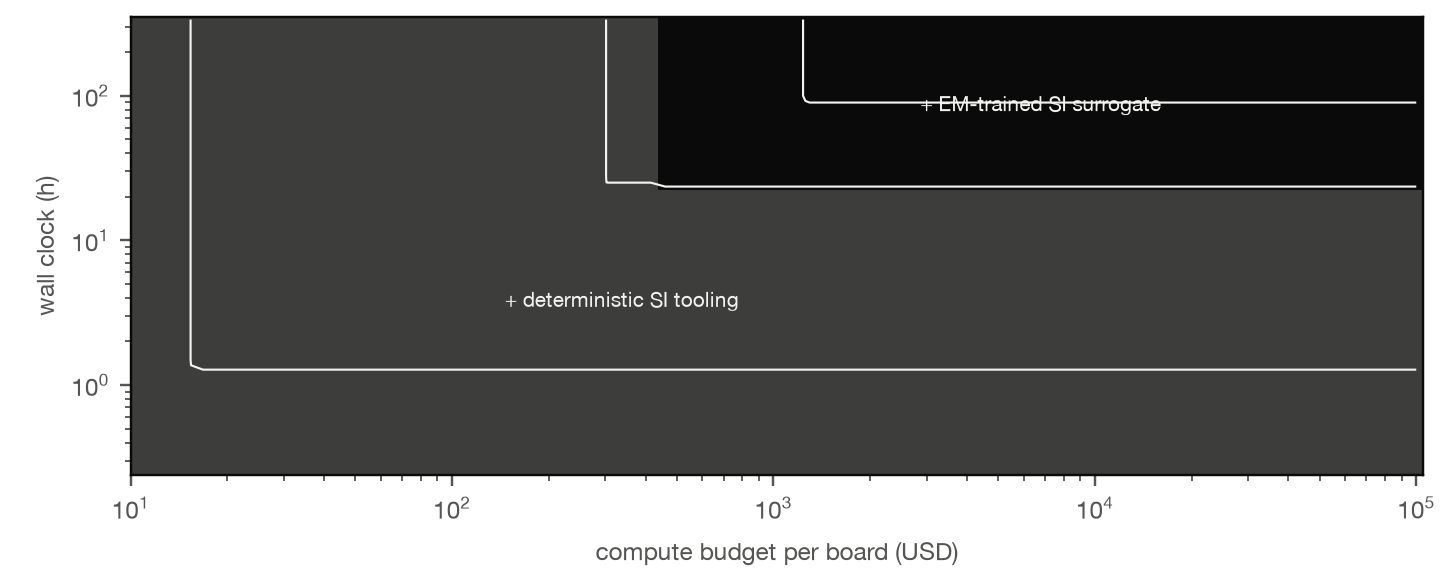
\includegraphics[width=0.36\linewidth]{fig/fc_winner_hard.png}
\caption{Forecast reward on the hard tier (DDR5-class board). Left: best achievable reward over seven strategies against budget and wall clock. Right: the strategy that achieves it.}
\label{fig:surface}
\end{figure}

\begin{table}[t]
\centering\small
\forecasttable
\caption{Forecast reward (medium / hard tier) by budget per board and wall clock.}
\label{tab:fc}
\end{table}

Three implications follow. Routing candidates are cheap---about one cent of CPU for a medium board---so budgets above about \$100 per board barely move simple search; the binding constraints are wall clock and evaluator fidelity. Strategies that improve the evaluator (deterministic SI tooling and EM-trained surrogates) are the only ones whose ceiling rises with spend. RL, with a fixed cost of several thousand dollars and days, reaches less than search within the horizons considered. These are forecasts, not results; the benchmark exists to replace them with measurements.

\section{Limitations}
The set has eight boards from one design house, which limits stylistic diversity. The boards are public and may appear in model training data; the coincidence signal $F$ detects literal copying but not memorised style. The reward uses geometric proxies for SI; it does not yet run full-wave simulation, which gerber2ems makes possible on sampled nets. Length groups are approximated by net class. Baselines ran under emulation on one machine and will be repeated on native hardware. Placement is held fixed; placement tasks are future work.

\section{Conclusion}
Routing a board and routing it right are different problems, and the second has lacked a public measuring stick. Using fabricated open boards as gold masters turns the claims of self-improving layout systems into numbers anyone can reproduce. We invite submissions of agents, routers and learned methods.

\paragraph{Reproducibility.} Code, tasks, baselines, forecast parameters and this paper's figures are at \url{https://github.com/elevenarms/pcb-gold-eval}; \texttt{make all} rebuilds them from pinned inputs.

\paragraph{Acknowledgements.} The gold-master boards are Antmicro's open-hardware designs. Research for this paper was assisted by AI agents; all citations were verified against primary records.

\bibliographystyle{plainnat}
\bibliography{refs}
\end{document}
